
% Carsten: Add a connection to chapter 3 in this intro.

The latest technological breakthrough in gesture-sensing devices has come in the form of a Leap Motion Controller (Leap Motion, San Francisco, CA, United States). 
The controller, approximately the size of a box of matches, allows for the precise and fluid tracking of multiple hands, fingers, and small objects in free space with 
sub-millimeter accuracy~\citep{Guna2014}. This chapter is based on the Leap Motion Controller documentation for the Orion software (i.e version 3.2 of the Leap motion software), 
and aims to highlight the important conceptual foundation for using the Leap Motion Controller in this thesis' design review application.

\section{Physical properties}
The Leap Motion Controller (see fig.~\vref{fig:leapmotion} and~\vref{fig:leapmotion2}) contains two stereoscopic cameras, with a field of view of about 150 degrees, 
in addition to three infrared LEDs. These infrared lights periodically emit light pulses with a wavelength of 850 nanometer, and thus outside the visible light spectrum. 
During the light pulses, 
which light up about eight cubic feet in front of the controller, grayscale stereo images are captured by the cameras and sent to the 
Leap Motion tracking software~\citep{LeapMotion2016}. 
This image capturing has an effective range from approximately 25 to 600 millimeters above the device.
In the software, the images are analyzed to reconstruct a 3D representation of what the device sees, 
compensating for static background objects and ambient environmental lighting. 
The Leap Motion software combines this sensor data with an internal model of the human hand to help cope with challenging tracking conditions.


\begin{figure}%[h!] %[H]
	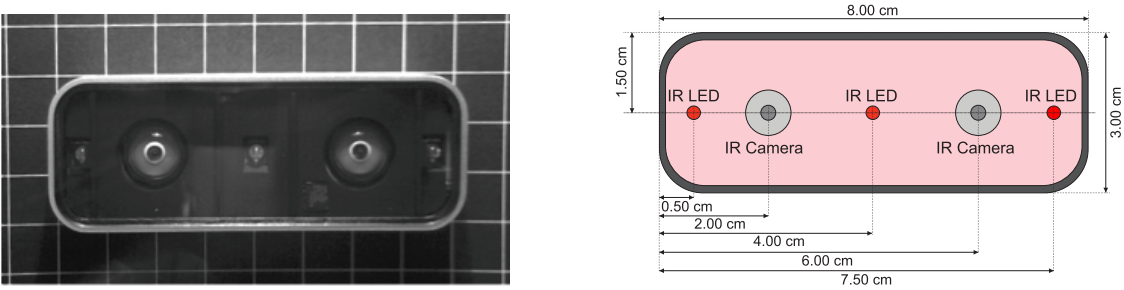
\includegraphics[width=\linewidth]{pictures/LMC_measures.png}
	\caption[Visualization of a Leap Motion Controller]{Visualization of a Leap Motion Controller, with Infrared Imaging (left) and a Schematic View (right)~\citep{Weichert2013}.}
	\label{fig:leapmotion2}
\end{figure} 

\section{The Leap API}
The controller itself can be accessed and programmed through high level Application Programming Interfaces (APIs), with support for a variety of programming languages, 
including C++, C\#, Objective-C, Java, JavaScript and Python. Although the API is programmed almost exclusively in C, access through a variety of other languages 
is achieved by virtue of various "wrapper libraries", which exposes and translates functions from their respective languages into the corresponding C function[cite].
In addition to this, the Leap Motion SDK also features integration with commercial game engines such as Unity and the Unreal Engine~\citep{Guna2014}. 
This section will cover important concepts in the Leap API, which are thoroughly used in the thesis implementation.

\subsection{Integration with the Unity editor}
To use Leap Motion in a Unity project one simply import the Leap Motion Asset Package, which included plugin files, as well as hand prefabs, scripts and demo scenes, 
into the project and includes certain components to the scene (the most important being the LeapHandController and HandModels prefabs). LeapHandController is responsible
for representing the Leap Motion device in the Unity scene, while the HandModels prefabs are model of the virtual hands that are to mimic what the user's hands are doing.  


\subsection{The hand abstractions}
The Leap Motion API offers many convenient abstractions for relevant properties when detecting and tracking hands.
Hands are the main entity tracked by the Leap Motion controller, and it maintains an inner model of the human hand and validates the data from 
its sensors against this model. This allows the controller to track finger positions even when some fingers are not visible from the Leap Motion Controllers point of view.

The Hand class represents a physical hand detected by the Leap, and is perhaps one of the most central abstractions in the Leap Motion API. 
A Hand object provides access to lists of its pointables as well as attributes describing the hand position, orientation, and movement.
Each hand-object have object-representations for its fingers, palm etc, each with its own data.
One common way to access the hands are through the Frame object, which is an object-oriented representation of the last captured frame of the device.
Each frame will contain a list called "hands", which will contain a hand-object per detected and tracked hand.
These hands have their own characteristics, which are handily available to the developer. 
Some examples (from~\citet{LeapMotion2016}) of what variables the hand objects contain include:

\begin{itemize}
\item isRight, isLeft — Whether the hand is a left or a right hand.
\item Palm Position — The center of the palm measured in millimeters from the Leap Motion origin.
\item Palm Velocity — The speed and movement direction of the palm in millimeters per second.
\item Palm Normal — A vector perpendicular to the plane formed by the palm of the hand. The vector points downward out of the palm.
\item Direction — A vector pointing from the center of the palm toward the fingers.
\item grabStrength, pinchStrength — Describe the posture of the hand.
\item Motion factors — Provide relative scale, rotation, and translation factors for movement between two frames.
\end{itemize}

Below is an example derived from the MovementController.cs class in the Design Review implementation (in C\#). 
This examples highlights how hand-object can be acquired from the frame-object, how we can e.g.~make sure its a left-hand
before proceeding, and how we can calculate a new player model position based on the hand position offset from the gesture origin.
Note that this code is incomplete and only meant as a somewhat compact example:

\begin{table}
\label{table:annotation_visibility_code}
\lstset{style=csharp}
\begin{lstlisting}

//Update() runs every frame (typically between 30 - 120 times per second)
void Update()
{
    Frame frame = LeapBehavior.getLastFrame();
    iBox = frame.InteractionBox; //Used for normalization
    for (int i = 0; i < frame.Hands.Count; i++)
    {
        Hand hand = frame.Hands[i]; 

        if (hand.IsLeft && leftHand.getGestureType() != HandState.NONE)
        {
            //Measure hand position from palm position
            Vector leapPoint = hand.StabilizedPalmPosition;
            
            //Converting from right hand to left hand coordinate convention
            leapPoint.z *= -1.0f; 

            //Normalizing the point
            Vector normPoint = iBox.NormalizePoint(leapPoint, false);
            
            if (gestureHand.getGestureType() == HandState.PALM_DOWN) 
            {
                //PALM_DOWN is the gesture to navigate up and down the y-axis          
                //The y-axis hand offset from origin:
                float y_offset = normPoint.y - gestureHand.GetGestureOriginPosition().y;

                //Calculate new player model position
                transform.position += transform.up * speed * y_offset * Time.deltaTime;
            }             
        }
    }
}
\end{lstlisting}
\caption[Accessing the Leap Motion Frame objects]{Accessing the Leap Motion Frame objects}
\end{table}

\subsection{The coordinate system}
The Leap Motion API enables acquisition of the recognized object's position through Cartesian and spherical coordinate systems, 
which are used to describe positions in the controller's sensory space~\citep{Guna2014}. The hand positions above the Leap Motion device are given as three dimensional
vectors on the form \{x, y, z\}, with origin being in the center of the Leap Motion surface (see~\vref{fig:leapmotion3})~\citep{LeapMotion2016}.  
Positional information, like the position of a hand, or the position of the tip of a finger, can be access in various ways. One way is to access the hands through the
Frame-object, and then find the relevant hand, palm, finger or finger-joint.

The Leap Motion API uses a right-handed coordinate convention, meaning that when the user is positioned in front of the Leap Motion Controller the x-axis grows more positive 
towards the right, the y-axis grows more positive upwards and the z-axis grows more positive towards the user (see~\vref{fig:leapmotion3}). 
As frameworks like that of Unity uses a left-handed convention for its coordinate system, i.e that the z-axis grows more positive away from the 
user instead of towards, the Leap Motion API also does an appropriate convention to adhere to its software environment. 
The Leap Motion API also adhere to differences in units, as e.g Unity uses a default unit of meters, while the Leap Motion uses millimeters~\citep{LeapMotion2016}.

\begin{figure}%[h!] %[H]
	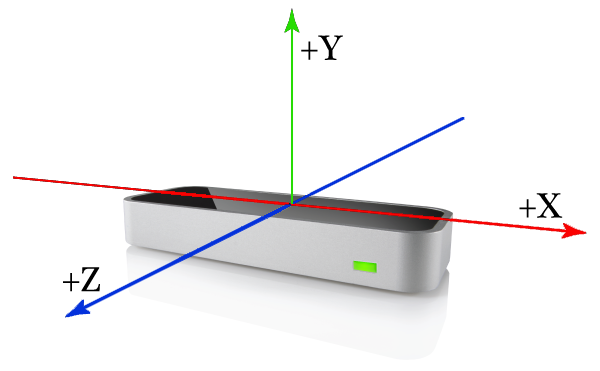
\includegraphics[width=\linewidth]{pictures/Leap_Axes.png}
	\caption[Leap Motion Coordinates]{The Leap Motion Coordinate System has its origin between the two cameras.}
	\label{fig:leapmotion3}
\end{figure} 

\subsection{The detection utilities}
To provide a common and high level interface to recognize gestures the Leap Motion API offers several detection utilities called \textbf{\textit{detectors}}.
Detectors are scripts in the core asset package that serve as basic building blocks for hand action detections, and can e.g.~detect whether a certain finger is extended or not
or which way the palm is facing~\citep{LeapMotion2016}. New detectors can also be created by the developer by extending
the Detector base class and implement logic that calls "Active" when the detector turns on and "Deactivate" when it turns off.

Several of these detector can be chained together using a \textbf{\textit{Logic Gate}} to create more complex expressions. 
The Detector Logic Gate is itself a detector that logically combines two or more other detectors, using operations like AND, OR, NAND (not AND) and NOR (not OR), 
to determine its own state.
If one thus were to make a thumb's up-gesture, one could use a logic gate with an AND-configuration together with a detector for detecting whether or not the
thumb is extended and a detector for determining whether or not the thump if facing upward~\citep{LeapMotion2016}. 

The detectors also have some public variables, which can be adjusted for preference. These include "Period", which determines how often the detector checks the hand state,
"Hand Model", which refers to which hand model is being observed and several "On and off values", which sets the thresholds for when the detector should be on (i.e the
detector recognizes the property it's looking for) or off. The latter is can especially be the subject of repeated adjustment, as it is deemed crucial to find a good
compromise between the two values (more on this in the implementation chapter). The detectors also has some public functions, with two of the most important ones being
"OnActivate" and "OnDeactivate". OnActivate is called by its detector when the detector turns on (activates), while OnDeactivate is called when it turns off (deactivates). 

This outlines the primary means of creating gestures and connecting them to actions using the Leap Motion API. One can create gesture expressions, like the thumb's up-gesture
described above, using a Logic Gate with AND. This Logic Gate will only be active (on), while all of the detectors it references ("is hooked up to") are active, so in our example
only when the thumb is extended AND facing upwards. By then assigning a custom created function, e.g.~a function called "Accept", to the Logic Gate's OnActive-function we
ensure that this function is called only when the thumb's up-gesture is done correctly. 



% Technically, very few details are publicly known about the precise nature of the algorithms used due to patent and trade secret restrictions.

% \section{Important Leap components}




% Hands, fingers, palm, directions, frames, interaction box etc. 
% See \\
% https://developer.leapmotion.com/documentation/csharp/devguide/Leap\_Overview.html\#motion-tracking-data \\
% https://developer.leapmotion.com/documentation/csharp/devguide/Leap\_Coordinate\_Mapping.html\#map3d \\
% https://developer.leapmotion.com/documentation/csharp/devguide/Leap\_Hand.html \\


% \section{Detectors - The building blocks of gesture recognition}
% The detector scripts. How they can be combined. Logic gates. 
% See https://developer.leapmotion.com/documentation/unity/unity/Unity\_DetectionUtilities.html

% \section{Integration with the Unity editor}
% How the pieced fit together. How the stuff is organized (e.g the modules).
% See https://developer.leapmotion.com/documentation/unity/index.html